\section{Resultados}
\subsection{Pantallas del sistema y su funcionamiento}
\label{pantallas}

\subsubsection{Pantalla del módulo de Conversion y Carga de Archivos}
Esta vista es la primera que se ve al ingresar al sistema, consta de dos partes independientes, 

\paragraph{Formulario de documentos e imágenes}
En la Figura \ref{fig:vista-modulo-conversion} se observa el formulario que usa el sistema para cargar los documentos y convertirlos a PDF o cargar una imágen para almacenarla en la nube y posteriormente hacer su codigo QR. Es importante que el sistema maneje varios tipos de datos ya que así lo requiere la institución.
\begin{figure}[!tbh]
    \centering
    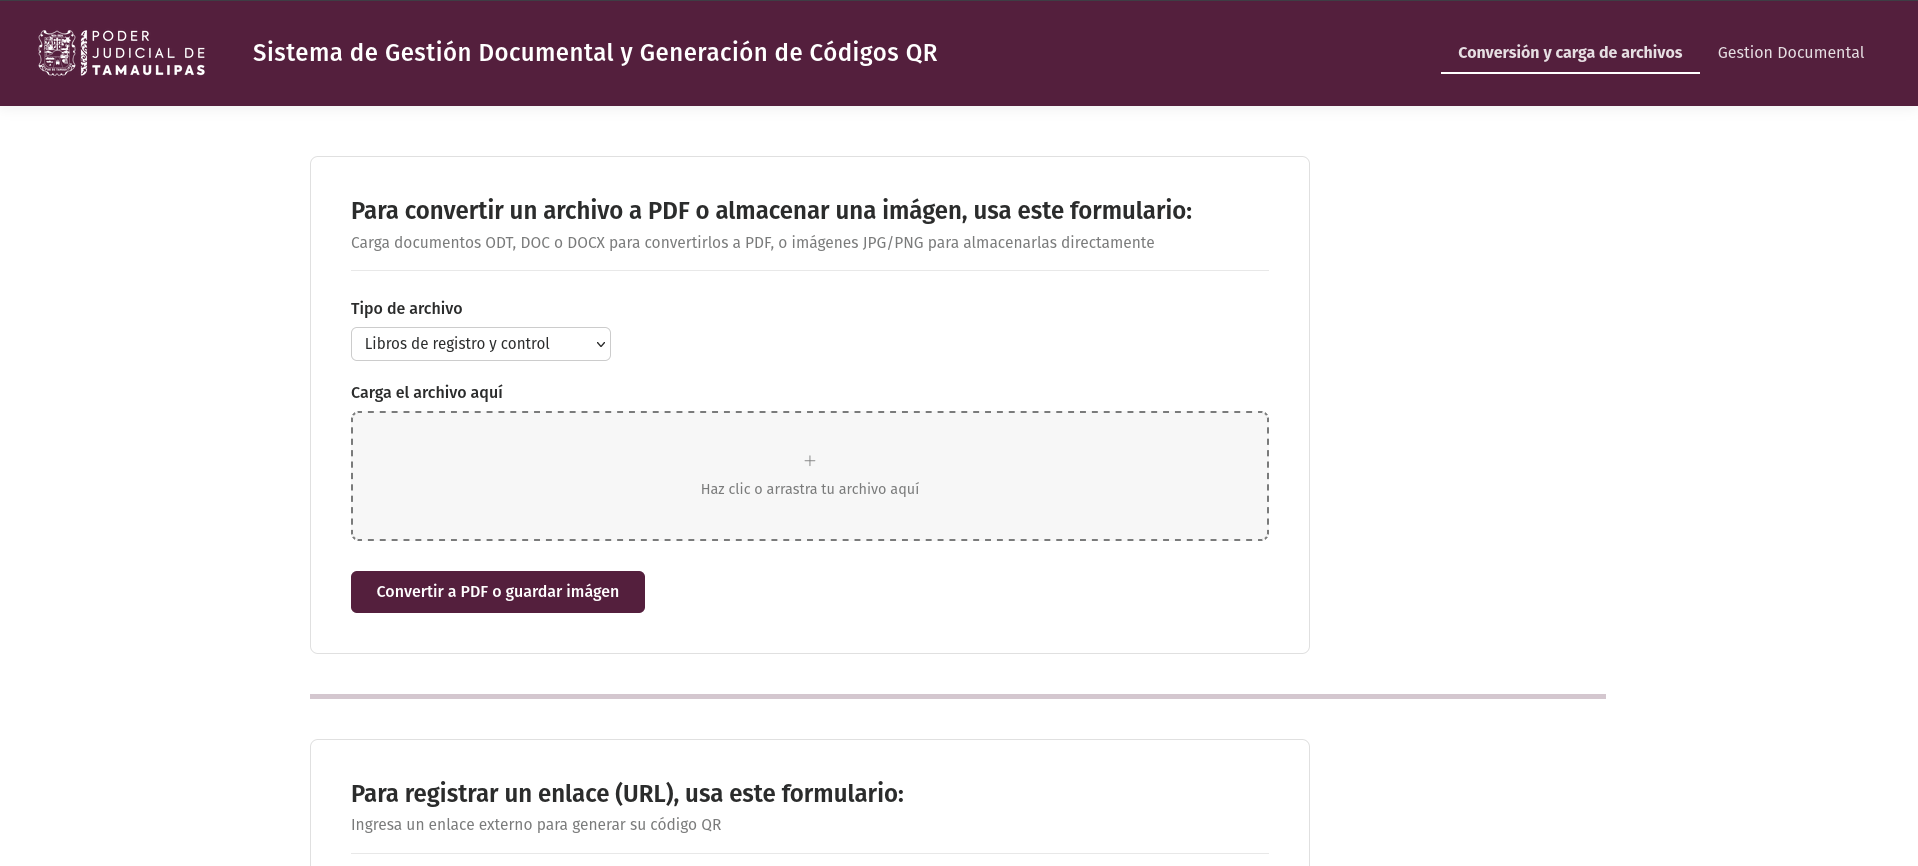
\includegraphics[width=0.9\linewidth]{img/vista-modulo-conversion.png}
    \caption{Interfaz del módulo de conversion y carga de documentos e imágenes. Fuente: elaboración propia}
    \label{fig:vista-modulo-conversion}
\end{figure}


Este módulo cambia de acuerdo al estado en el que se encuentre el proceso de almacenamiento, en la Figura \ref{fig:modulo-conversion-archivo-cargado} se puede observar como cambia la interfaz al cargar un archivo, indicando que se ha cargado correctamente al formulario y el nombre del archivo, para que el usuario pueda comprobar que es el archivo deseado, y continuar con el último paso que es darle click al botón para convertir y almacenar su docuemento.
\begin{figure}[!tbh]
    \centering
    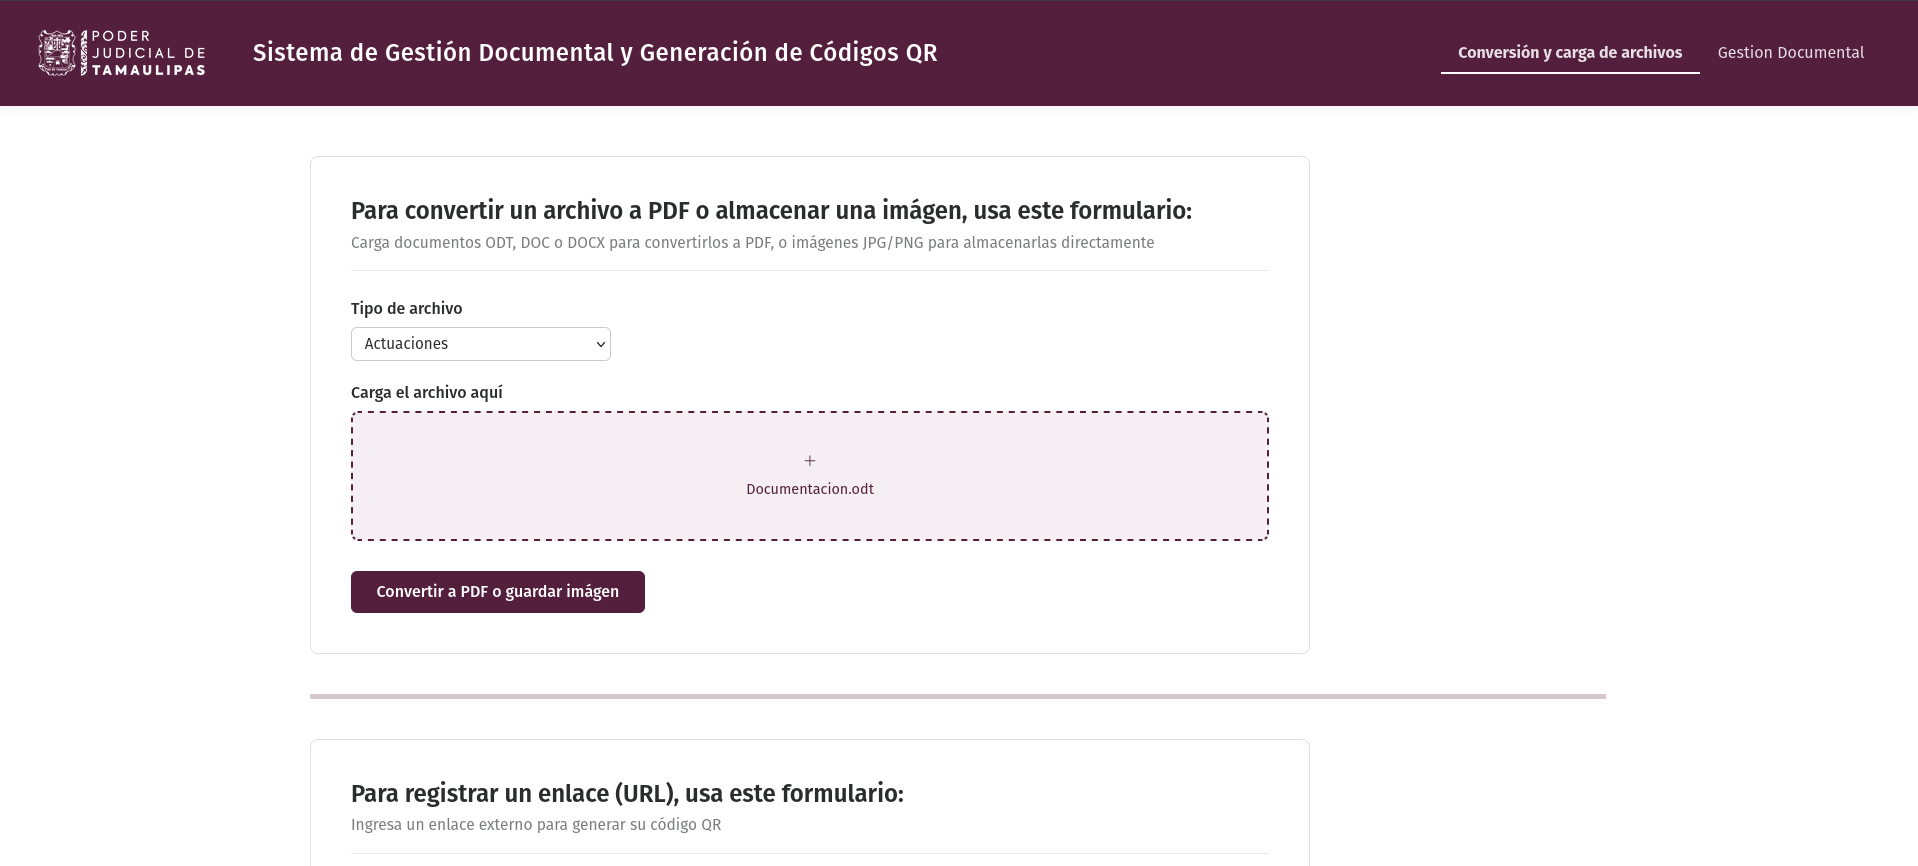
\includegraphics[width=0.9\linewidth]{img/modulo-conversion-archivo-cargado.png}
    \caption{Interfaz del módulo al cargar un archivo. Fuente: elaboración propia}
    \label{fig:modulo-conversion-archivo-cargado}
\end{figure}

Al presionar el botón y cuando la carga del archivo ocurre sin ningpun problema, el sistema muestra un mensaje, como se ve en la Figura \ref{fig:mensaje-documento-almacenado}, indicando que el archivo esta almacenado correctamente y ya puede verlo en la lista de documentos almacenados en el sistema.
\begin{figure}[!tbh]
    \centering
    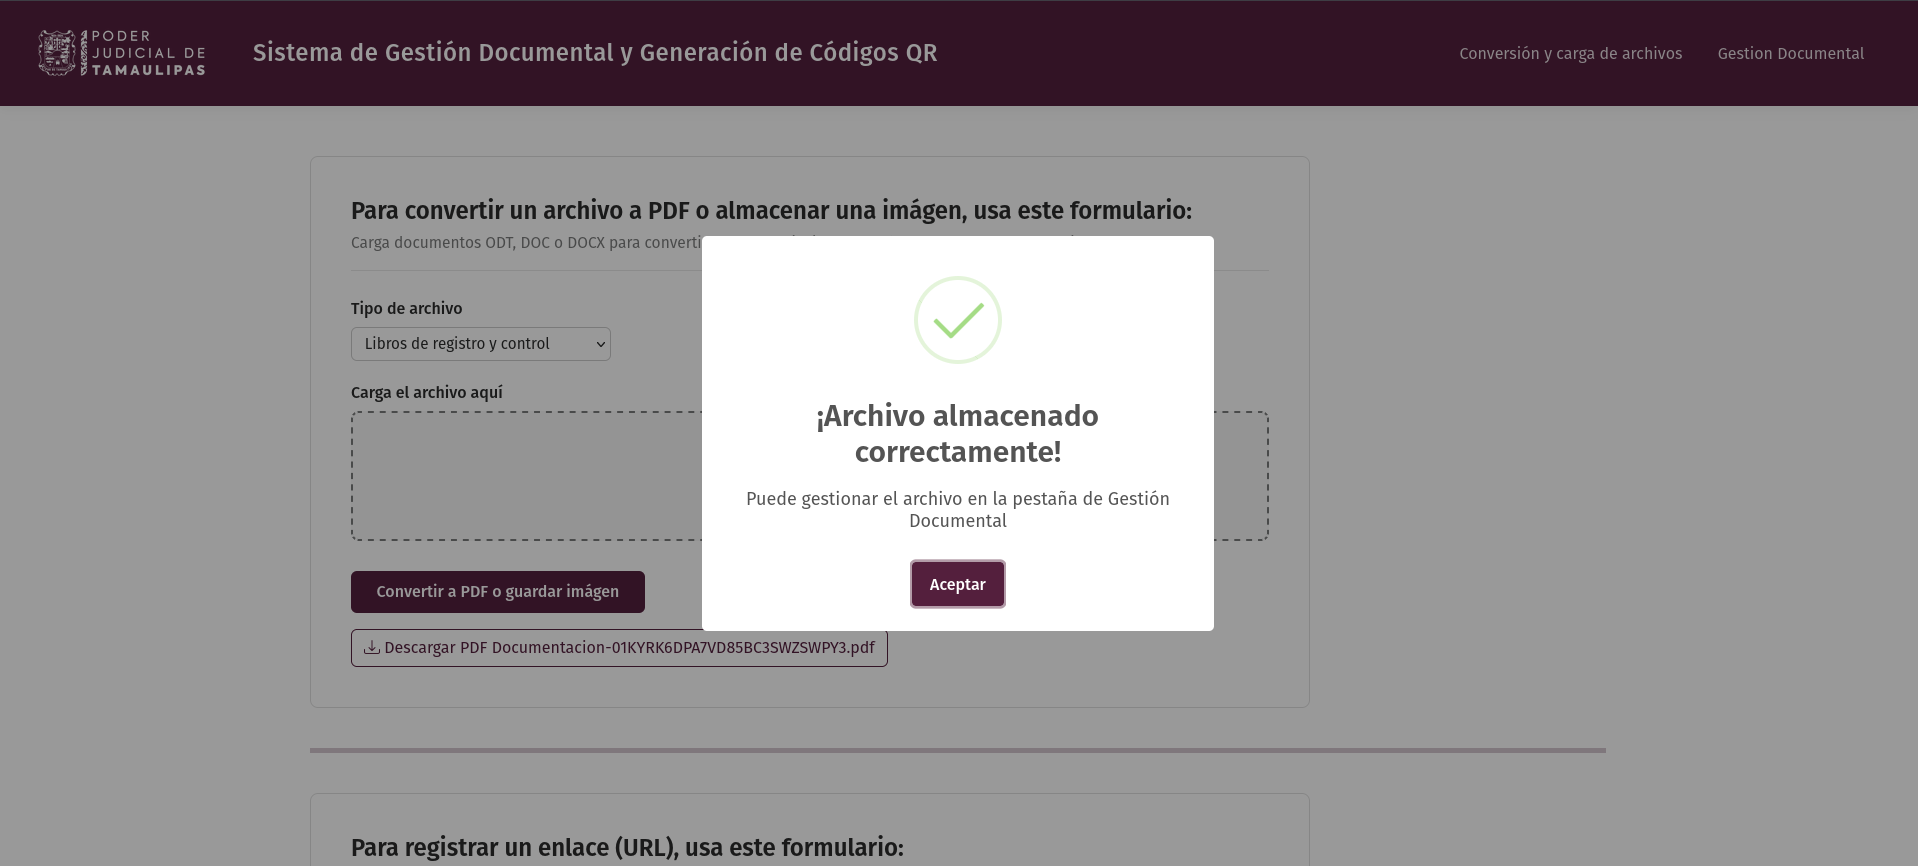
\includegraphics[width=0.9\linewidth]{img/mensaje-documento-almacenado.png}
    \caption{Mensaje al cargar un archivo con éxito. Fuente: elaboración propia}
    \label{fig:mensaje-documento-almacenado}
\end{figure}

Al aceptar el mensaje de la figura \ref{fig:mensaje-documento-almacenado}, el sistema muestra un botón, justo debajo del botón de conversión, que facilita la descarga de los archivos en formato PDF, esto por si el usuario solo queria hacer la conversión a ese formato, sin la necesidad de visitar el módulo de Gestión Documental en ese momento.
\begin{figure}[!tbh]
    \centering
    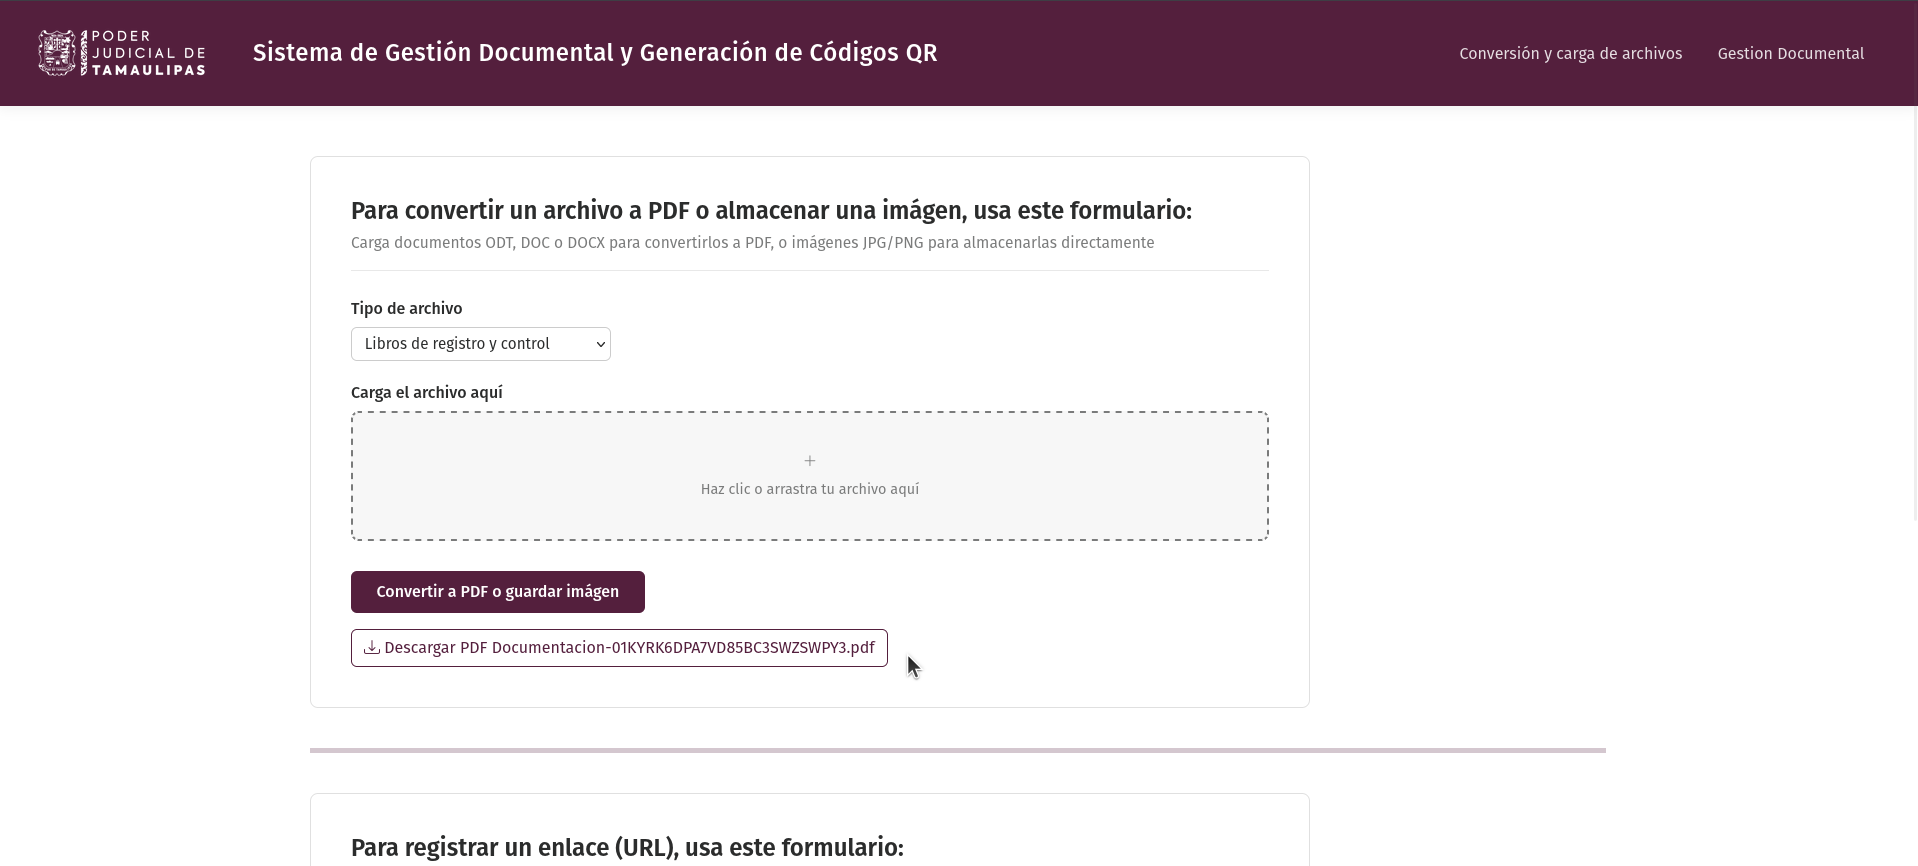
\includegraphics[width=0.9\linewidth]{img/vista-despuesde-almacenar-archivo.png}
    \caption{Botón para descargar el documento recién convertido a PDF Fuente: elaboración propia}
    \label{fig:vista-despuesde-almacenar-archivo}
\end{figure}

\paragraph{Formulario de URL}
La segunda parte del módulo de conversión y carga de archivos, es el formulario de carga de URL, este sirve para poder guardar un enlace y cuando se necesite crear su codigo QR. Se junta con ambos procesos ya que es usual que el personal requiere referenciar un sitio o página web en un documento, entonces esta funcionalidad facilita el pegar un enlace, guardarlo y después ir al módulo de gestión Documental y generar su codigo QR.

En la imagen \ref{fig:vista-modulo-url} se observa el formulario para almacenar una URL, este se encuentra debajo del formulario de conversion de archivos.
\begin{figure}[!tbh]
    \centering
    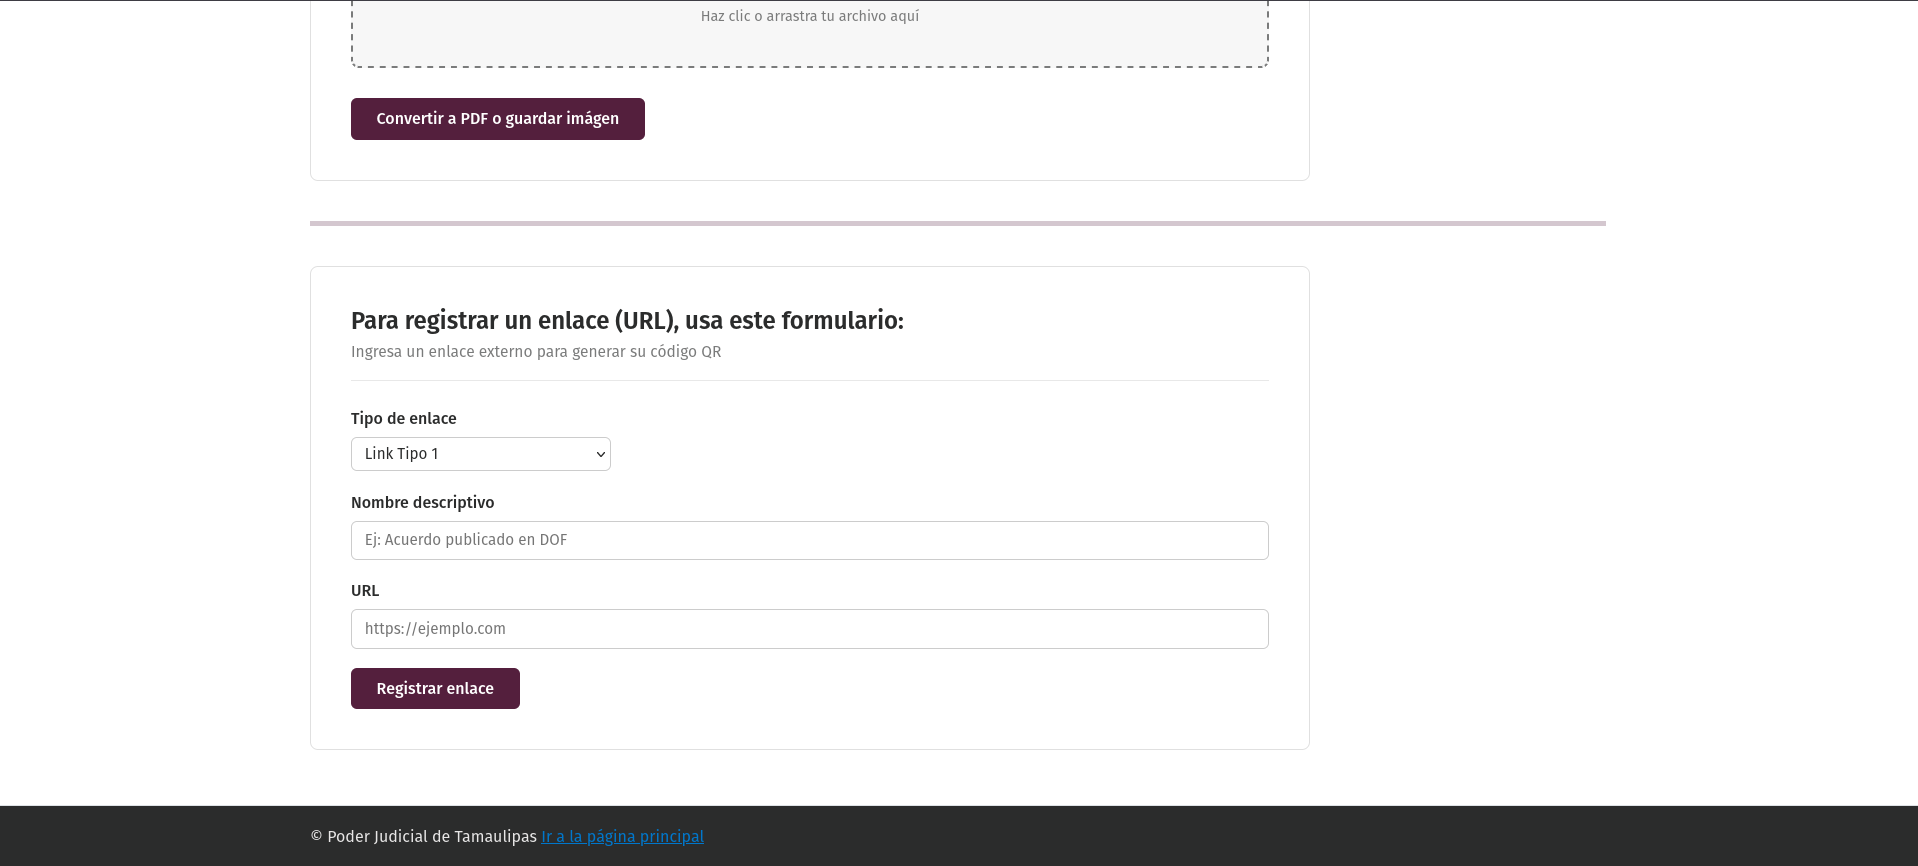
\includegraphics[width=0.9\linewidth]{img/vista-modulo-url.png}
    \caption{Interfaz del formulario para subir URLs. Fuente: elaboración propia}
    \label{fig:vista-modulo-url}
\end{figure}

El sistema también muestra un mensaje de éxito cuando se ha guardado correctamente, y le dice al usuario que hacer para obtener el QR.
\begin{figure}[!tbh]
    \centering
    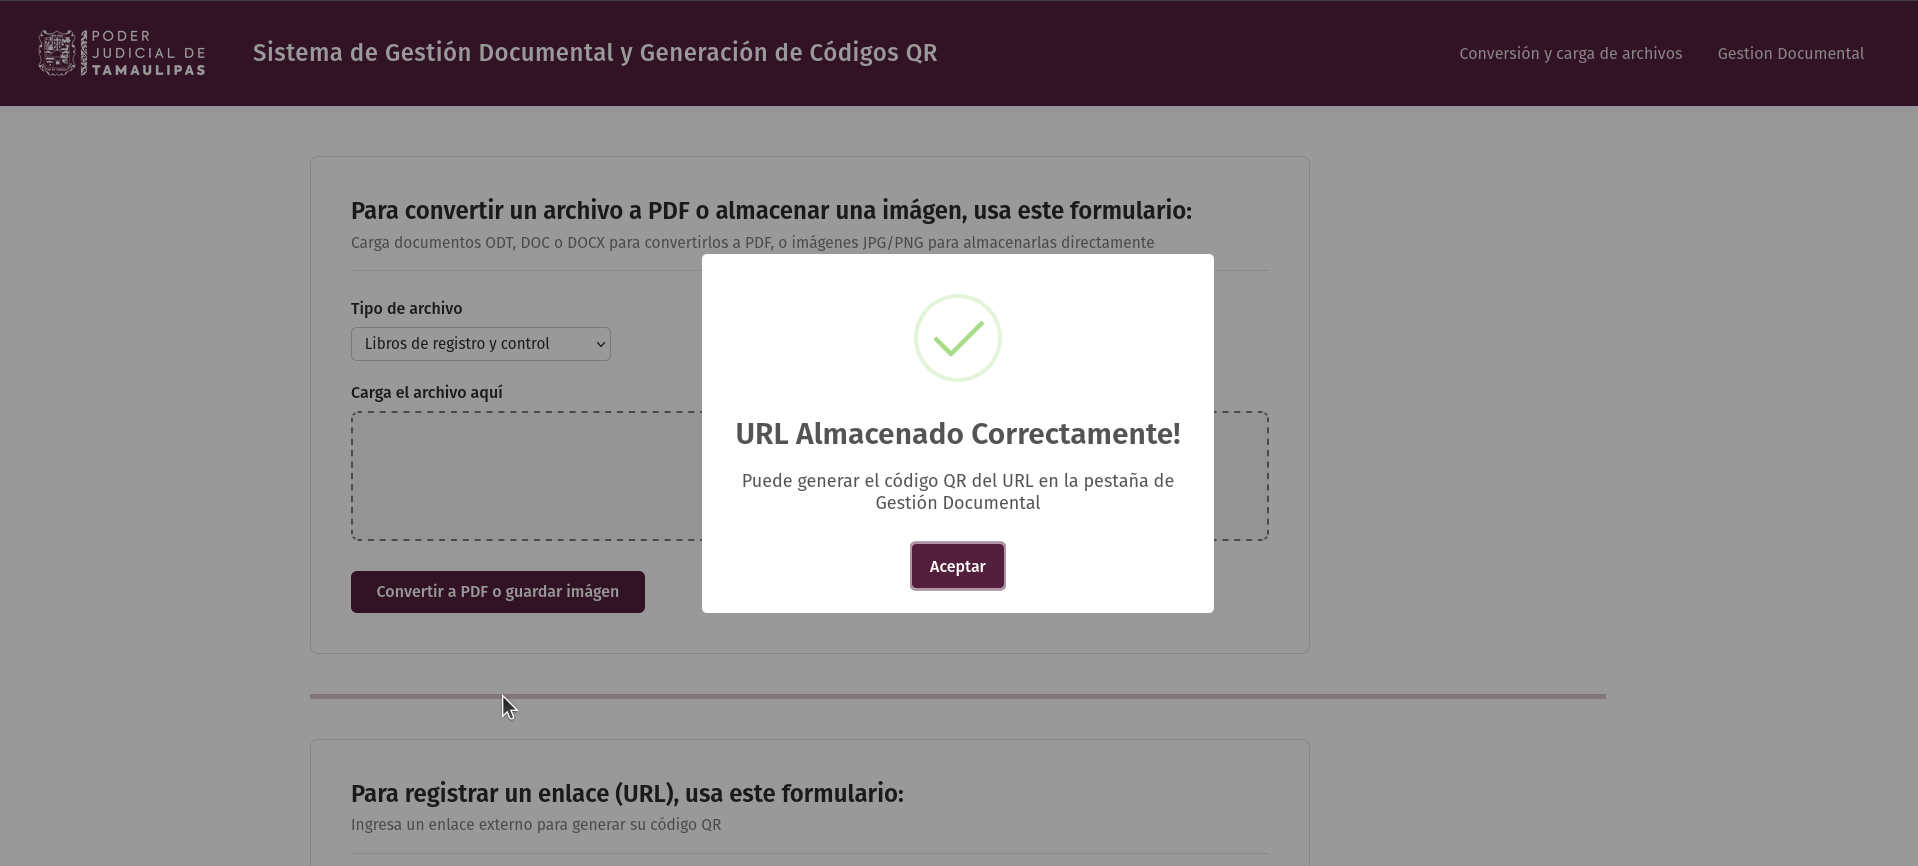
\includegraphics[width=0.9\linewidth]{img/mensaje-url-almacenado.png}
    \caption{Mensaje al cargar un URL con éxito. Fuente: elaboración propia}
    \label{fig:mensaje-url-almacenado}
\end{figure}

\subsubsection{Pantalla del modulo de Gestión Documental}
El segundo módulo del sistema es el de Gestión Documental, mostrado en la Figura \ref{fig:vista-gestion-documental}, el cual consta de una tabla con todos los archivos, ya sean documentos, imágenes o enlaces, listados por orden de creación, que es la fecha en que fueron cargados al sistema, al lado derecho de cada archivo se observan cuatro botones con las distintas acciones para cada uno de ellos.
Arriba de la tabla de archivos, esta un filtro para buscar con fácilidad por áreas de la organización o por tipo de documento, esto es la categoria que se le asigna al momento de que el usuario lo carga en el formulario de la pestaña de conversión y carga de archivos. También tiene una barra de búsqueda, para buscar archivos por nombre.
\begin{figure}[!tbh]
    \centering
    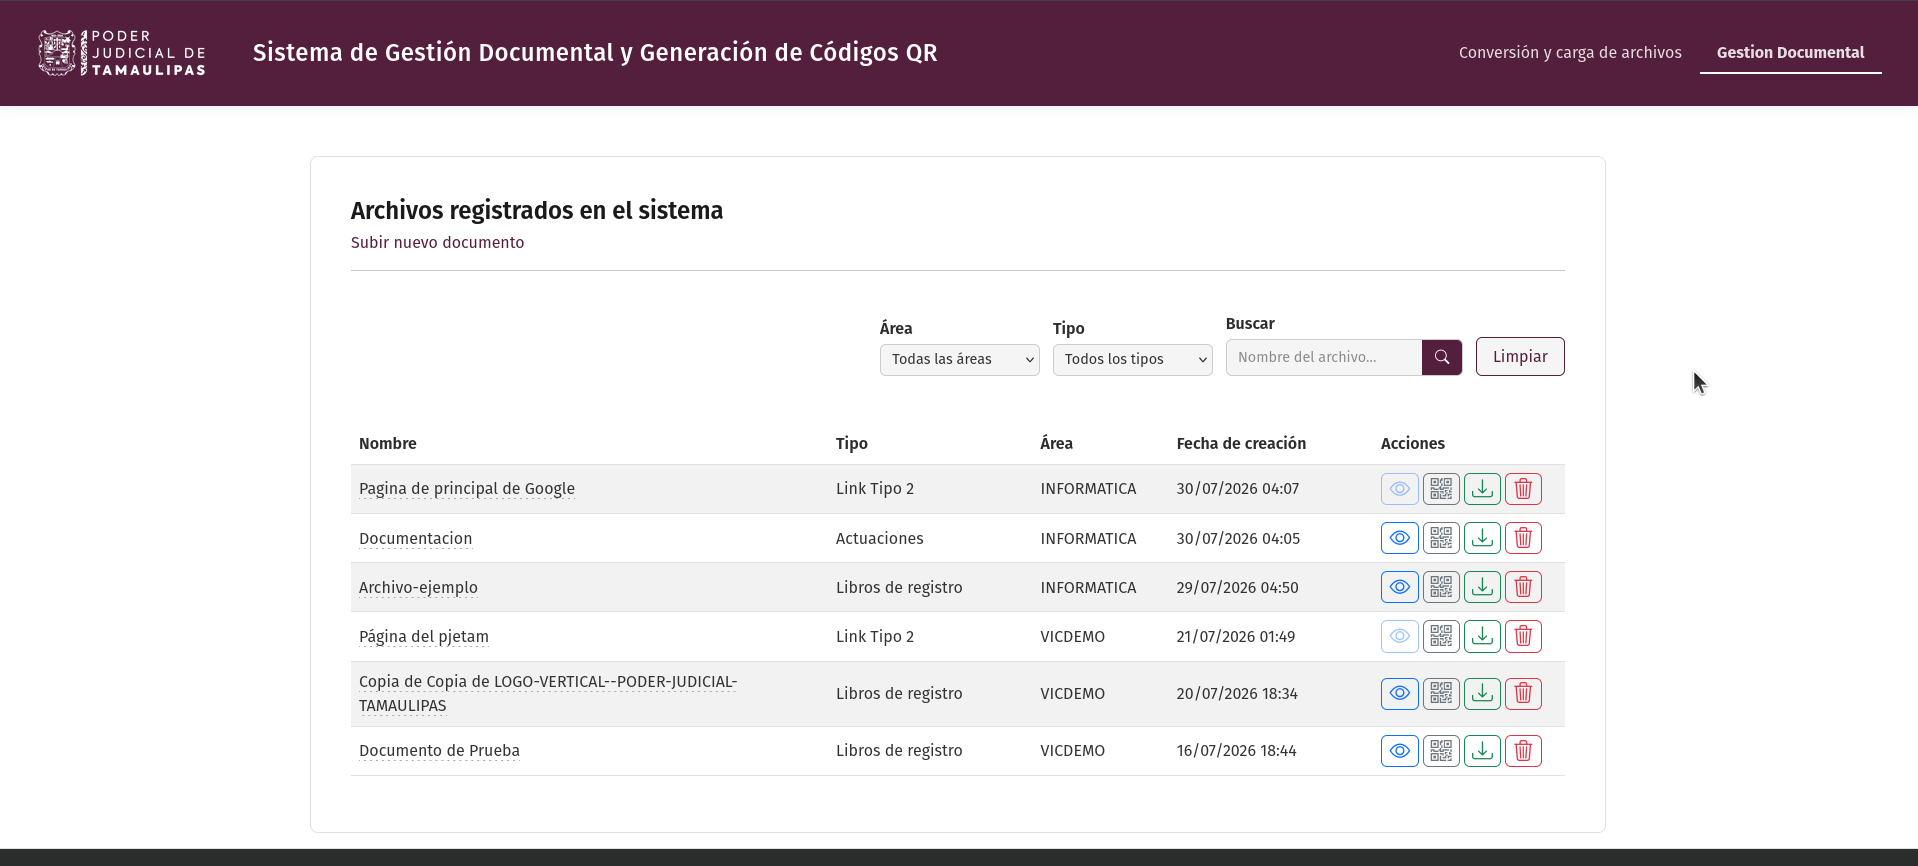
\includegraphics[width=0.9\linewidth]{img/vista-gestion-documental.png}
    \caption{Interfaz del módulo de Gestión Documental. Fuente: elaboración propia}
    \label{fig:vista-gestion-documental}
\end{figure}

\begin{figure}[!tbh]
    \centering
    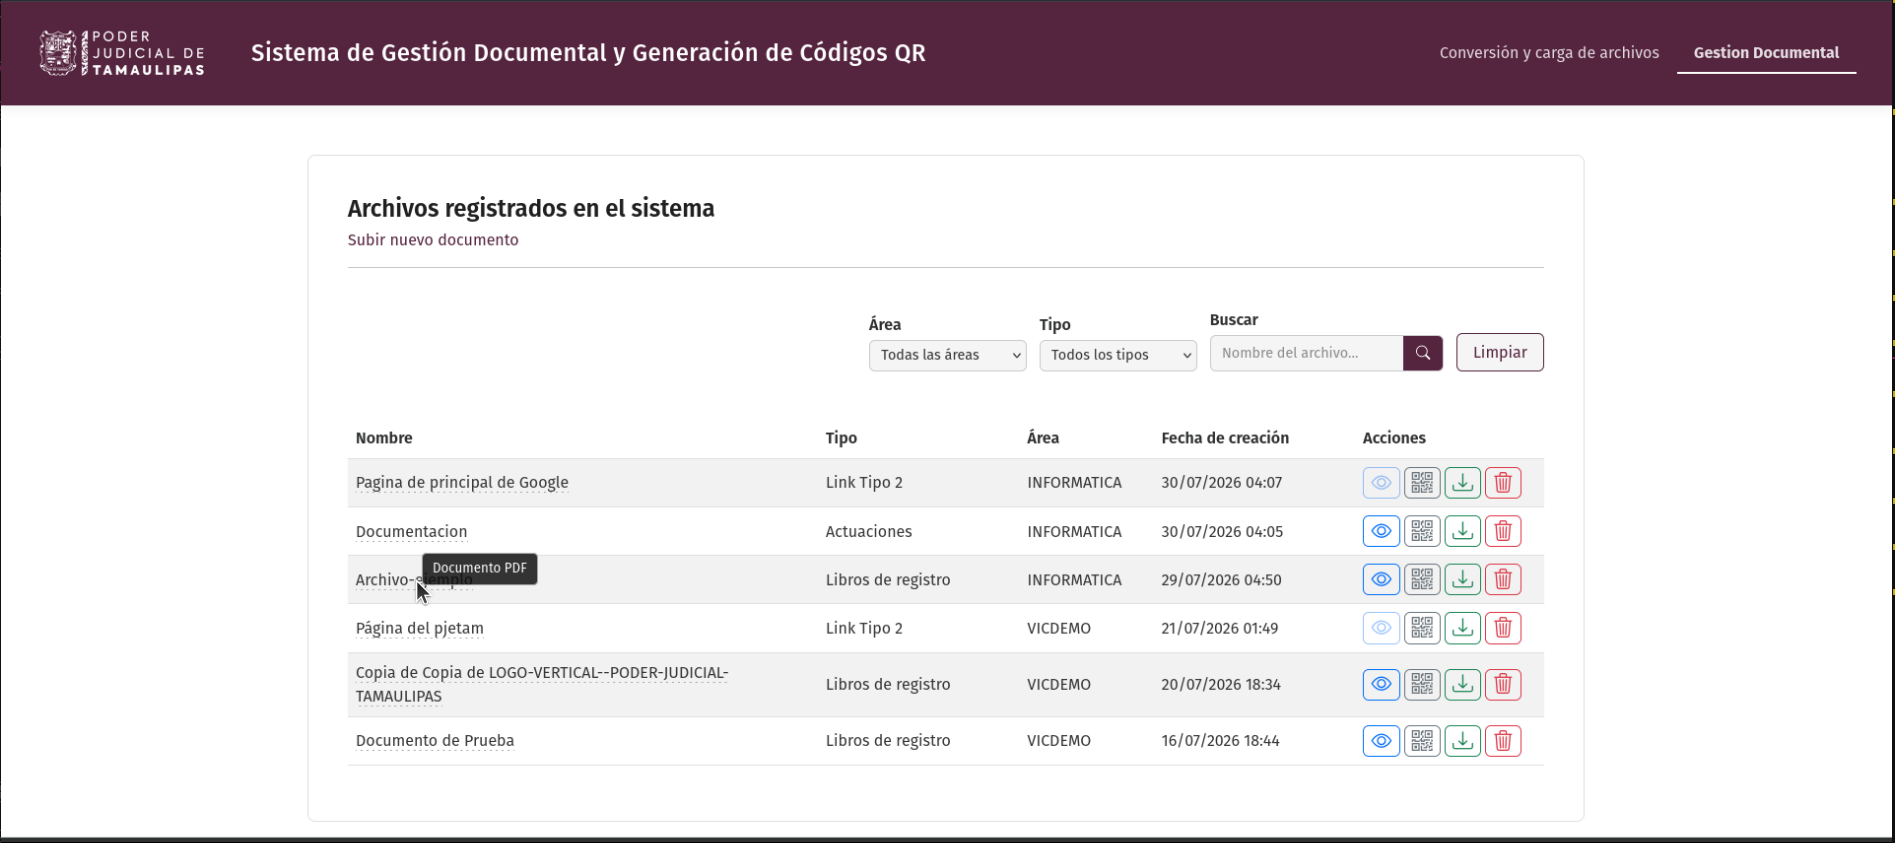
\includegraphics[width=0.9\linewidth]{img/gestion-cursor.doc.png}
    \caption{Mensaje para identificar que tipo de archivo es. Fuente: elaboración propia}
    \label{fig:gestion-cursor.doc}
\end{figure}

\paragraph{Vista de la tabla al aplicar un filtro}
\begin{figure}[!tbh]
    \centering
    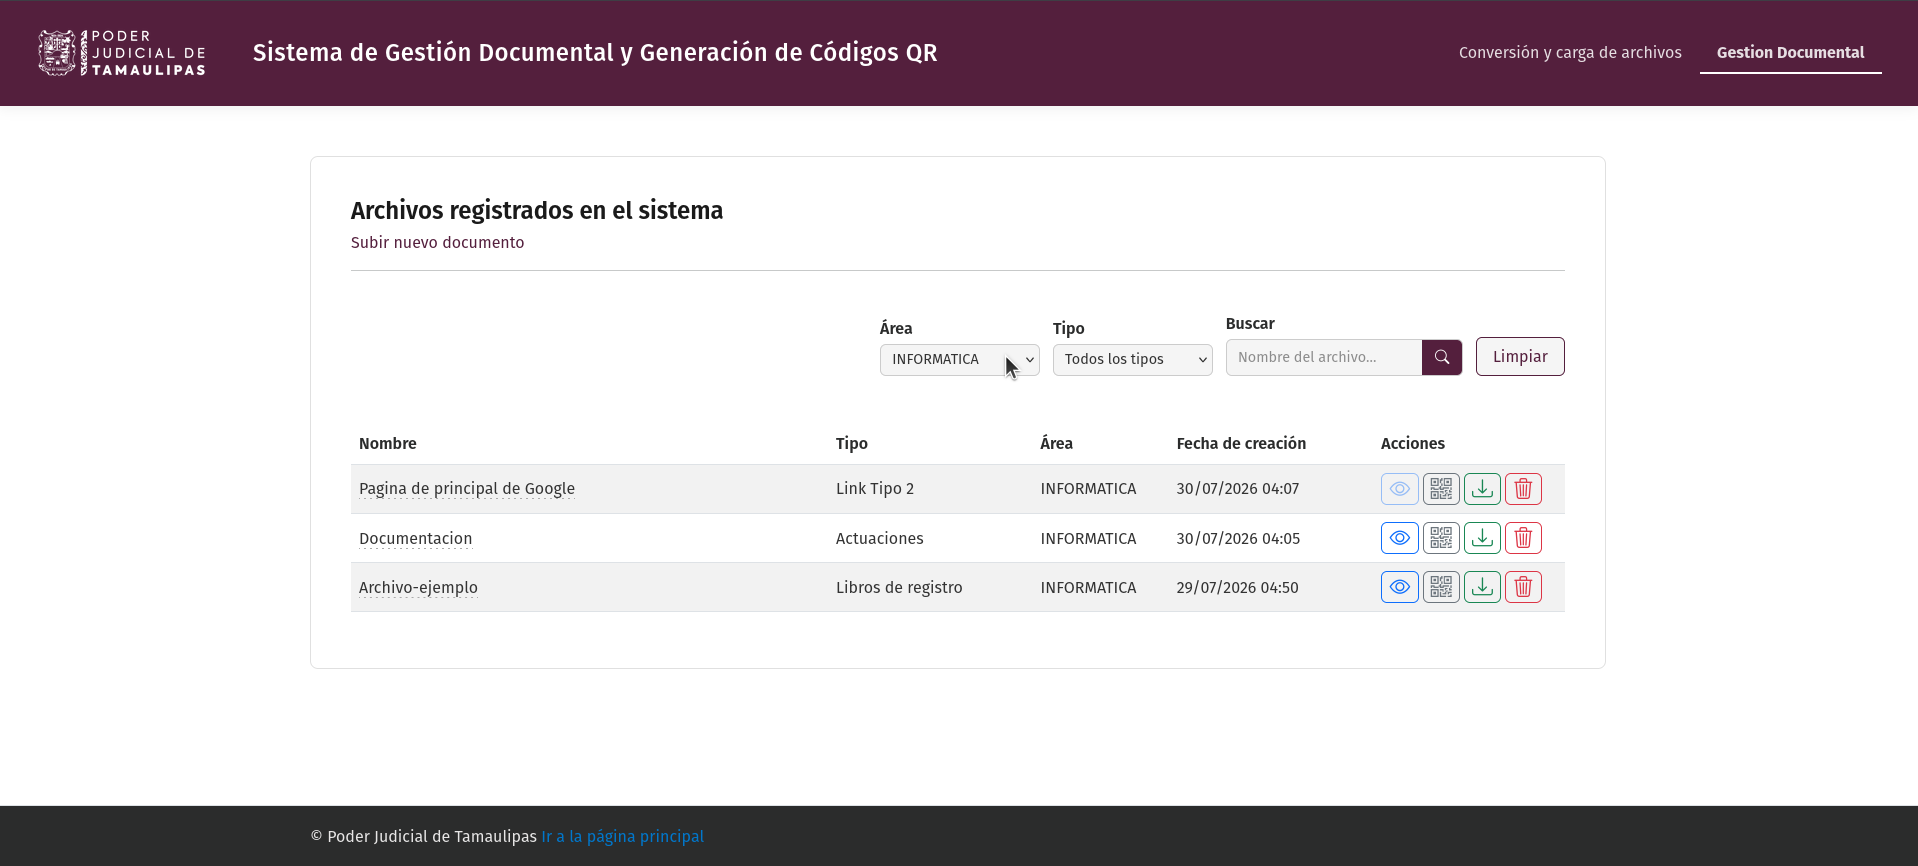
\includegraphics[width=0.9\linewidth]{img/vista-despuesde-busqueda-gd.png}
    \caption{Interfaz del módulo de Gestión Documental al aplicar un filtro. Fuente: elaboración propia}
    \label{fig:vista-despuesde-busqueda-gd}
\end{figure}



\paragraph{Vista al seleccionar la opción de visualizar un documento}
\begin{figure}[!tbh]
    \centering
    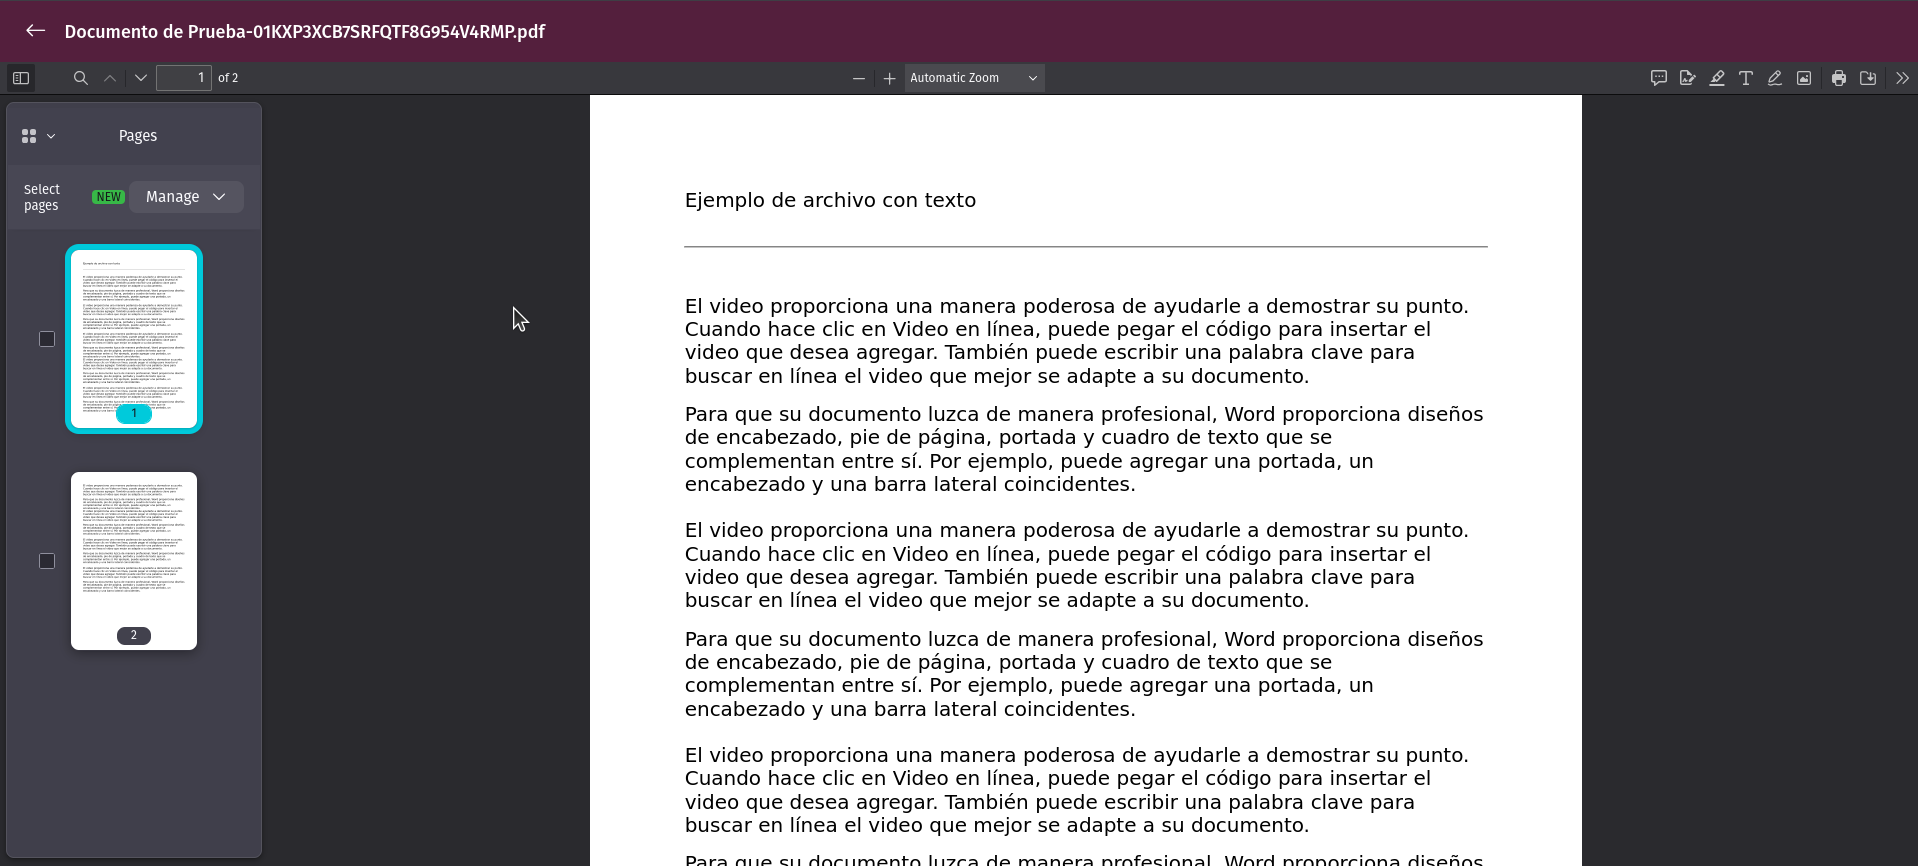
\includegraphics[width=0.9\linewidth]{img/vista-ver-doc.png}
    \caption{Interfaz al ver un documento desde Gestión Documental. Fuente: elaboración propia}
    \label{fig:vista-ver-doc}
\end{figure}


\paragraph{Vista al seleccionar la opción de visualizar una imagen}
\begin{figure}[!tbh]
    \centering
    
\includegraphics[width=0.9\linewidth]{img/vista-ver-imagen.png}
    \caption{Interfaz al ver una imágen desde Gestión Documental. Fuente: elaboración propia}
    \label{fig:vista-ver-imagen}
\end{figure}

\paragraph{Vista al generar un código QR}
\begin{figure}[!tbh]
    \centering
    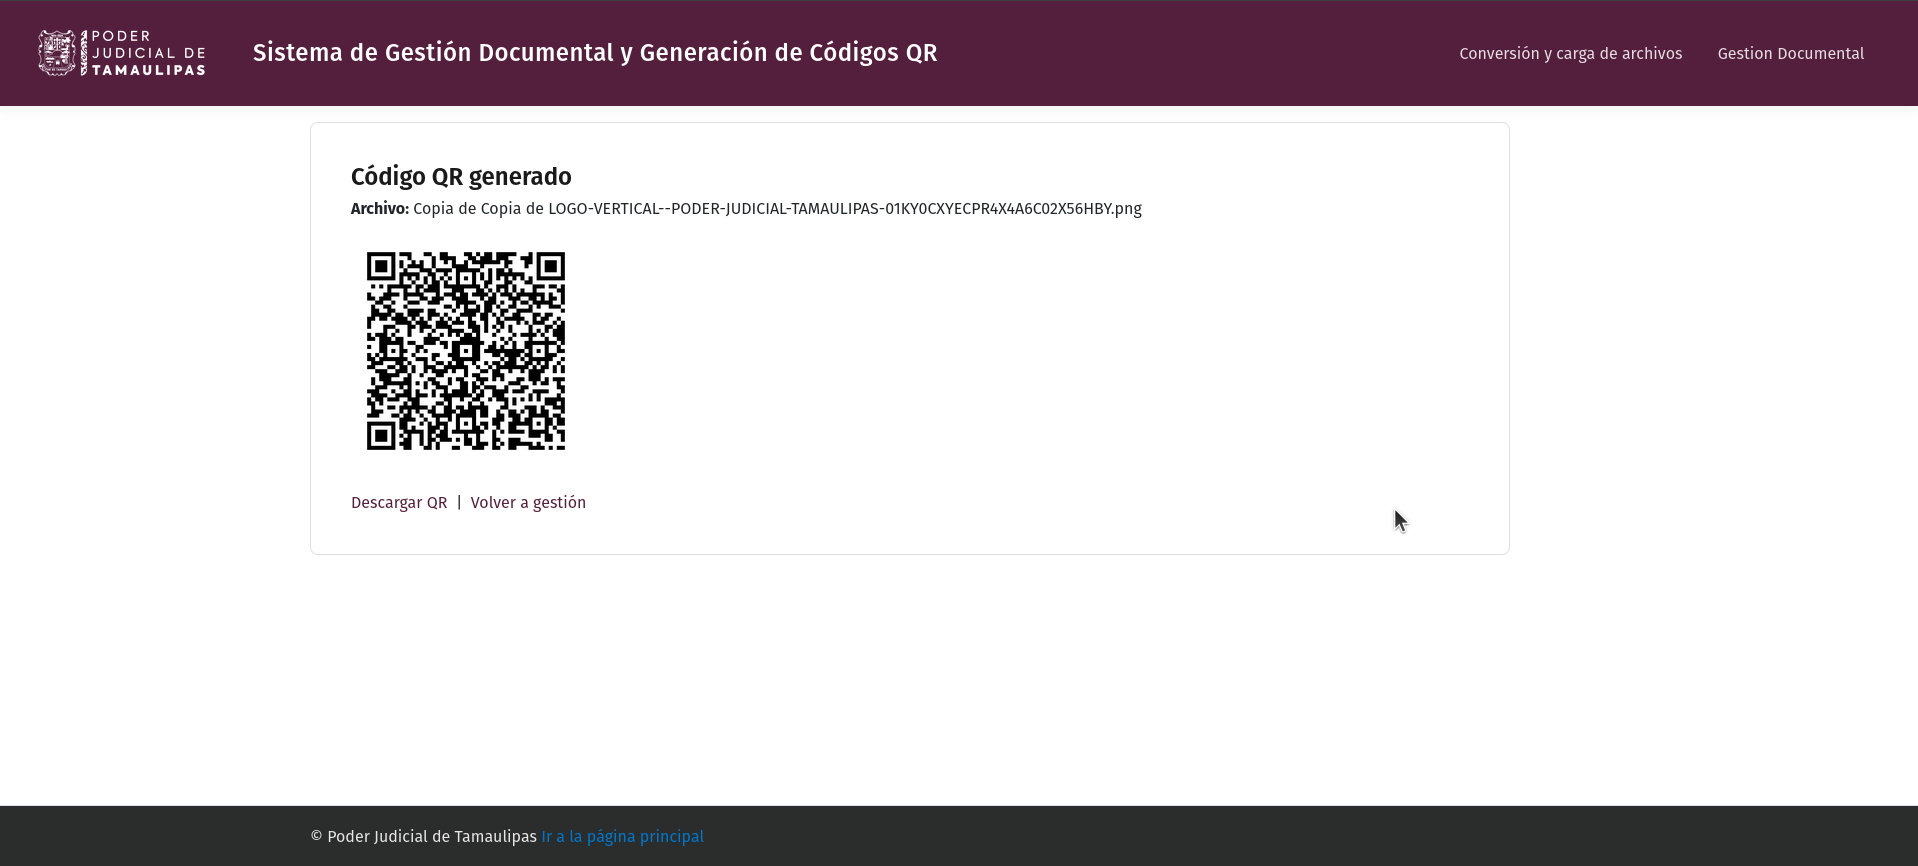
\includegraphics[width=0.9\linewidth]{img/vista-ver-qr-doc.png}
    \caption{Interfaz al generar el QR de un documento desde Gestión Documental. Fuente: elaboración propia}
    \label{fig:vista-ver-qr-doc}
\end{figure}

\paragraph{Vista al seleccionar la opción de eliminar un archivo}
\begin{figure}[!tbh]
    \centering
    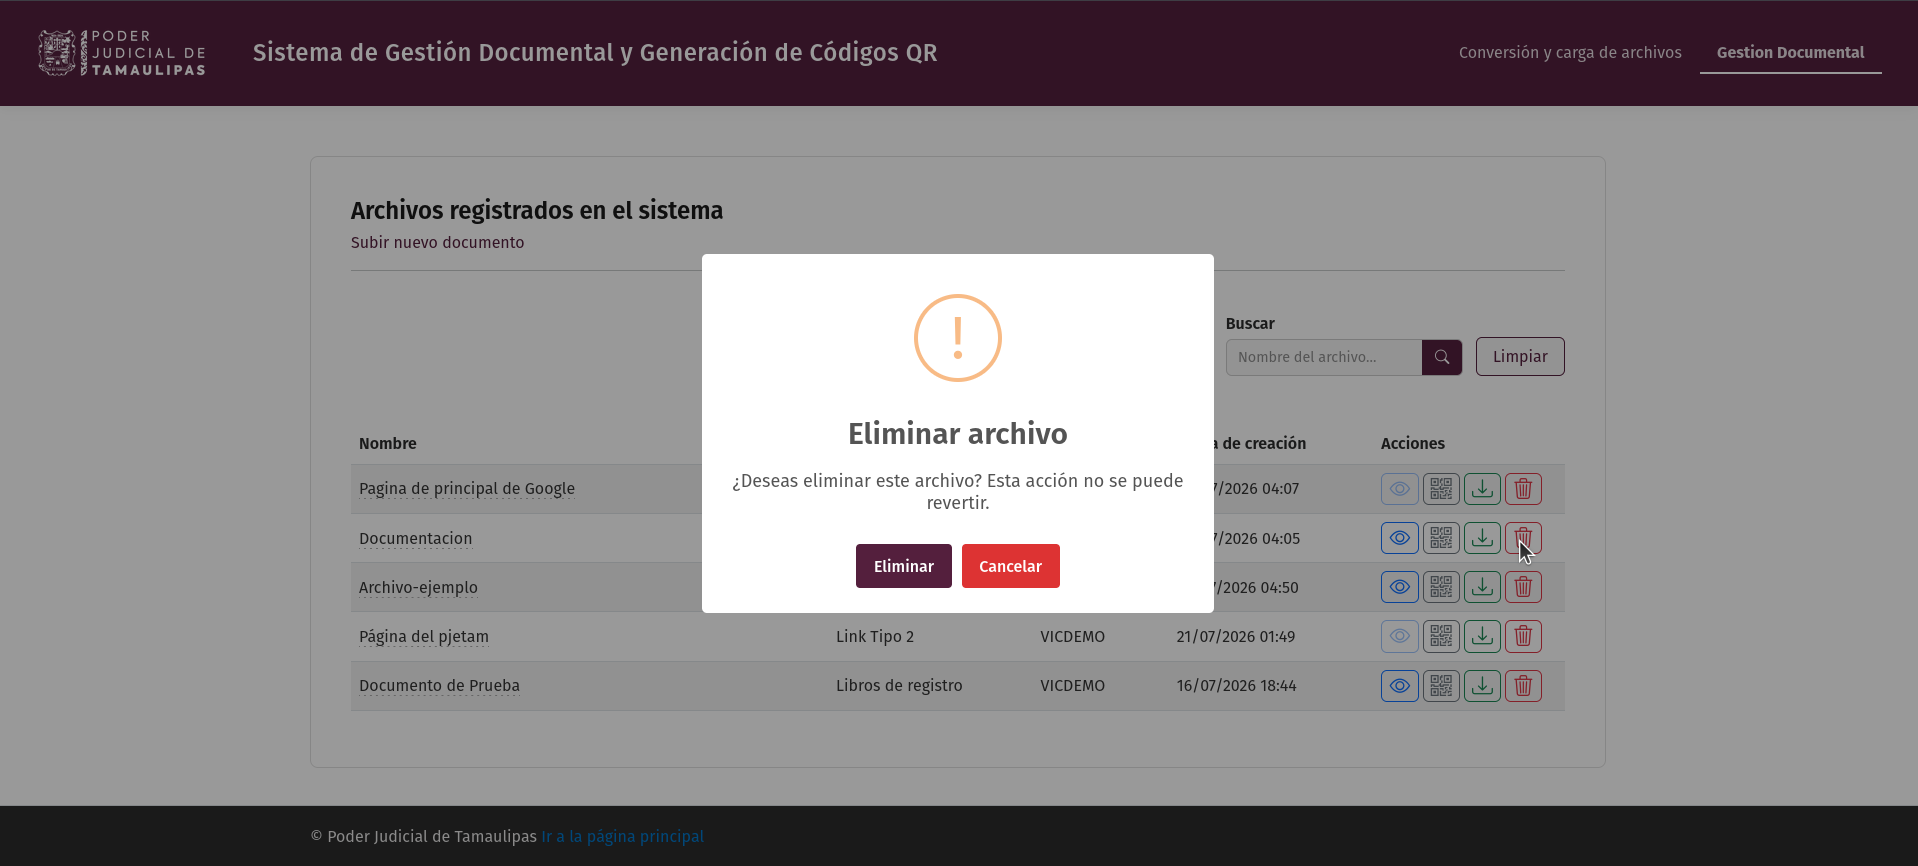
\includegraphics[width=0.9\linewidth]{img/vista-eliminar-doc.png}
    \caption{Interfaz al eliminar un documento desde Gestión Documental. Fuente: elaboración propia}
    \label{fig:vista-eliminar-doc}
\end{figure}

